\section{FuzzyLogic}
\begin{wrapfigure}{r}{0.4\textwidth}
    \vspace{-1.1cm}
    \begin{center}
      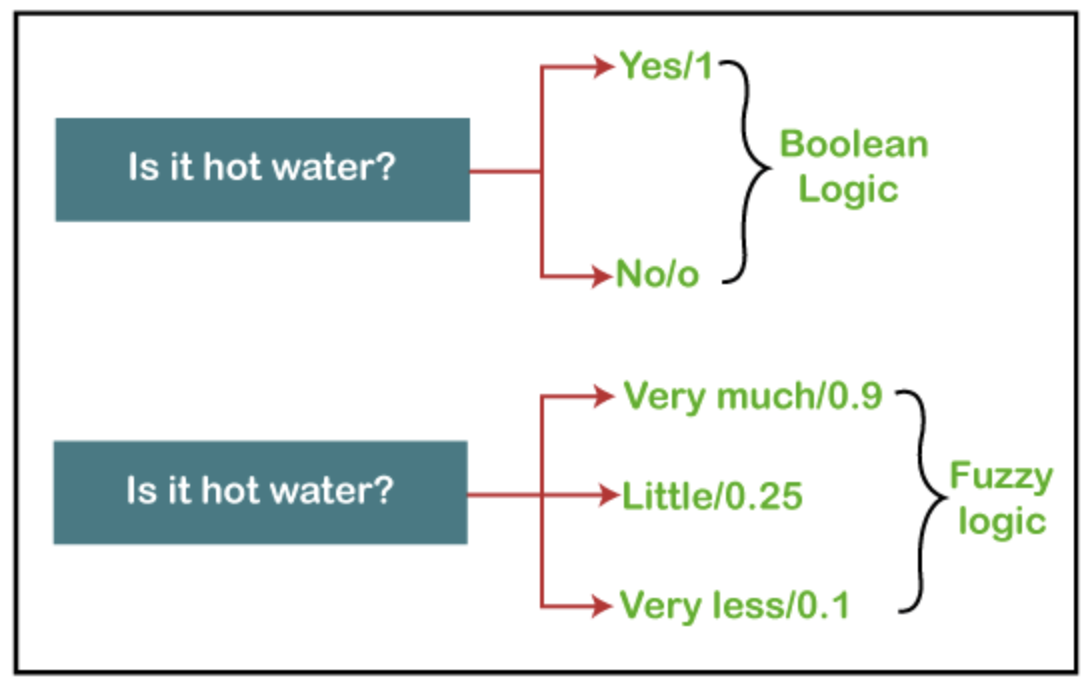
\includegraphics[width=0.4\textwidth]{FuzzyBoolLogic}
    \end{center}
    \vspace{-0.5cm}
    \caption{Vergleich von Fuzzy Logic zu Boolischer Logik \cite{FuzzyLogicGeeks}}
    \label{fig:FuzzyCompare}
    \vspace{-0.5cm}
  \end{wrapfigure}
Fuzzy Logic, erstmals in den 1960er Jahren von Lotfi Zadeh an der University of California entwickelt, stellt einen innovativen Ansatz der Datenverarbeitung dar, der auf Wahrheitsgraden basiert. Im Gegensatz zur herkömmlichen Booleschen Logik, die sich auf binäre Zustände von 1 oder 0 bzw. wahr oder falsch stützt, zeichnet sich die Fuzzy Logic durch ihre Fähigkeit aus, die Vielschichtigkeit von Zwischenzuständen zu berücksichtigen.\cite{FuzzyLogicTechTarget}\\
Das zentrale Merkmal der Fuzzy-Logik besteht darin, unpräzise Argumentationsweisen zu modellieren, die eine bedeutende Rolle in der bemerkenswerten Fähigkeit des Menschen spielen, unter Bedingungen der Ungewissheit und Ungenauigkeit rationale Entscheidungen zu treffen (Siehe Abbildung \ref{fig:FuzzyCompare}). Diese Fähigkeit basiert auf unserem Vermögen, aus einem Wissensbestand, der ungenau, unvollständig oder nicht völlig zuverlässig ist, ungefähre Antworten auf Fragen abzuleiten. Anders als in klassischen logischen Systemen strebt die Fuzzy Logic danach, die Grauzonen zwischen klaren Kategorien zu erfassen und somit eine flexiblere und menschlichere Art der Datenverarbeitung zu ermöglichen. Dieser Ansatz hat Anwendungen in verschiedenen Bereichen gefunden, darunter Steuerungssysteme, künstliche Intelligenz, Entscheidungsfindung und mehr. \cite{LoftiFuzzyLogic}

\subsection{Architektur eines Fuzzy Logic Systems}
Ein Fuzzy Logic Systems kann in vier Module unterteilt werden. Jede dieser Komponenten spielt dabei eine entscheidende Rolle für das gesammte System. 
Abbildung \ref{fig:FuzzyLogicArchitektur} zeigt den Aufbau eines Fuzzy Logic Systems auf.\\
Die Umwandlung der Systemeingänge ist Aufgabe des \textit{Fuzzification} Moduls. Dabei werden exakten Werte in sogenannte Fuzzy-Sets umgewandelt. Die \textit{Inference Engine} bestimmt anschließend den Grad der Übereinstimmung des aktuellen Fuzzy-Sets in Bezug auf jede Regel und trifft eine Entscheidung darüber, welche Regeln gemäß dem Eingangsfeld ausgelöst werden sollen. Durch eine Kombination der Ausgelösten Regeln wird anschließend eine Steuerungsaktion formuliert. Das \textit{Defuzzification} Model wird im anschluss dazu verwendet, aus den durch die \textit{Interence Engine} erhaltenen Fuzzy-Setz, exakte Ausgangswerte zu erhalten.
Die \textit{Rule Base} umfasst eine Sammlung von Regeln und den \grqq{\textit{IF-THEN}} Bedungunen, welche im Vorfeld definiert und dem System bereitgestellt werden. Diese werden verwendet, um das Entscheidungssystems auf Grundlage von linguistischen Variablen zu steuern. \cite{FuzzyLogicGeeks}\\
\vspace{-1cm}
\begin{center}
    \begin{figure}[h]
     \centering
     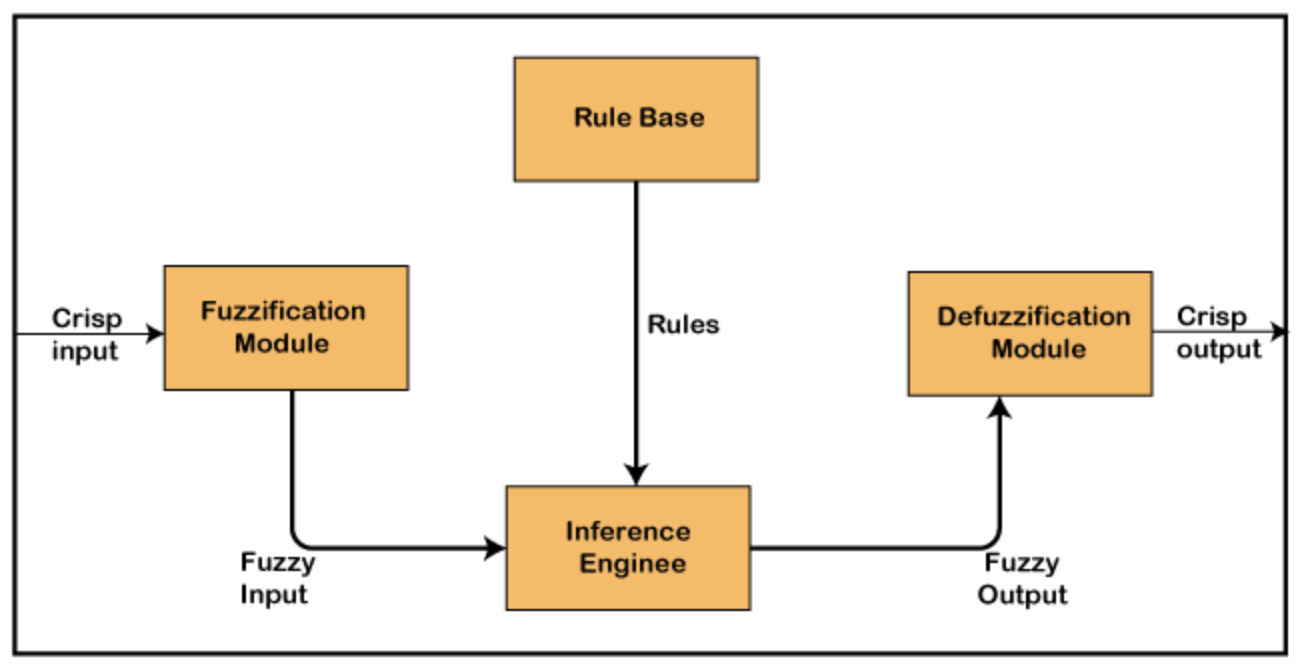
\includegraphics[width=0.8\textwidth]{FuzzyLogicArchitektur}
     \caption{Architektur eines Fuzzy Logic Systems \cite{FuzzyLogicGeeks}}
     \label{fig:FuzzyLogicArchitektur}
    \end{figure}
   \end{center}

